\documentclass[]{article}
\usepackage{lmodern}
\usepackage{amssymb,amsmath}
\usepackage{ifxetex,ifluatex}
\usepackage{fixltx2e} % provides \textsubscript
\ifnum 0\ifxetex 1\fi\ifluatex 1\fi=0 % if pdftex
  \usepackage[T1]{fontenc}
  \usepackage[utf8]{inputenc}
\else % if luatex or xelatex
  \ifxetex
    \usepackage{mathspec}
  \else
    \usepackage{fontspec}
  \fi
  \defaultfontfeatures{Ligatures=TeX,Scale=MatchLowercase}
\fi
% use upquote if available, for straight quotes in verbatim environments
\IfFileExists{upquote.sty}{\usepackage{upquote}}{}
% use microtype if available
\IfFileExists{microtype.sty}{%
\usepackage{microtype}
\UseMicrotypeSet[protrusion]{basicmath} % disable protrusion for tt fonts
}{}
\usepackage[margin=1in]{geometry}
\usepackage{hyperref}
\hypersetup{unicode=true,
            pdftitle={Project 2 : Explartion of Red Wine},
            pdfauthor={Isabel María Villalba Jiménez},
            pdfborder={0 0 0},
            breaklinks=true}
\urlstyle{same}  % don't use monospace font for urls
\usepackage{natbib}
\bibliographystyle{apsr}
\usepackage{graphicx,grffile}
\makeatletter
\def\maxwidth{\ifdim\Gin@nat@width>\linewidth\linewidth\else\Gin@nat@width\fi}
\def\maxheight{\ifdim\Gin@nat@height>\textheight\textheight\else\Gin@nat@height\fi}
\makeatother
% Scale images if necessary, so that they will not overflow the page
% margins by default, and it is still possible to overwrite the defaults
% using explicit options in \includegraphics[width, height, ...]{}
\setkeys{Gin}{width=\maxwidth,height=\maxheight,keepaspectratio}
\IfFileExists{parskip.sty}{%
\usepackage{parskip}
}{% else
\setlength{\parindent}{0pt}
\setlength{\parskip}{6pt plus 2pt minus 1pt}
}
\setlength{\emergencystretch}{3em}  % prevent overfull lines
\providecommand{\tightlist}{%
  \setlength{\itemsep}{0pt}\setlength{\parskip}{0pt}}
\setcounter{secnumdepth}{0}
% Redefines (sub)paragraphs to behave more like sections
\ifx\paragraph\undefined\else
\let\oldparagraph\paragraph
\renewcommand{\paragraph}[1]{\oldparagraph{#1}\mbox{}}
\fi
\ifx\subparagraph\undefined\else
\let\oldsubparagraph\subparagraph
\renewcommand{\subparagraph}[1]{\oldsubparagraph{#1}\mbox{}}
\fi

%%% Use protect on footnotes to avoid problems with footnotes in titles
\let\rmarkdownfootnote\footnote%
\def\footnote{\protect\rmarkdownfootnote}

%%% Change title format to be more compact
\usepackage{titling}

% Create subtitle command for use in maketitle
\newcommand{\subtitle}[1]{
  \posttitle{
    \begin{center}\large#1\end{center}
    }
}

\setlength{\droptitle}{-2em}
  \title{Project 2 : Explartion of Red Wine}
  \pretitle{\vspace{\droptitle}\centering\huge}
  \posttitle{\par}
  \author{Isabel María Villalba Jiménez}
  \preauthor{\centering\large\emph}
  \postauthor{\par}
  \predate{\centering\large\emph}
  \postdate{\par}
  \date{6 de diciembre de 2016}


\begin{document}
\maketitle

\begin{verbatim}
##  [1] "X"                    "fixed.acidity"        "volatile.acidity"    
##  [4] "citric.acid"          "residual.sugar"       "chlorides"           
##  [7] "free.sulfur.dioxide"  "total.sulfur.dioxide" "density"             
## [10] "pH"                   "sulphates"            "alcohol"             
## [13] "quality"
\end{verbatim}

\begin{verbatim}
##        X          fixed.acidity   volatile.acidity  citric.acid   
##  Min.   :   1.0   Min.   : 4.60   Min.   :0.1200   Min.   :0.000  
##  1st Qu.: 400.5   1st Qu.: 7.10   1st Qu.:0.3900   1st Qu.:0.090  
##  Median : 800.0   Median : 7.90   Median :0.5200   Median :0.260  
##  Mean   : 800.0   Mean   : 8.32   Mean   :0.5278   Mean   :0.271  
##  3rd Qu.:1199.5   3rd Qu.: 9.20   3rd Qu.:0.6400   3rd Qu.:0.420  
##  Max.   :1599.0   Max.   :15.90   Max.   :1.5800   Max.   :1.000  
##  residual.sugar     chlorides       free.sulfur.dioxide
##  Min.   : 0.900   Min.   :0.01200   Min.   : 1.00      
##  1st Qu.: 1.900   1st Qu.:0.07000   1st Qu.: 7.00      
##  Median : 2.200   Median :0.07900   Median :14.00      
##  Mean   : 2.539   Mean   :0.08747   Mean   :15.87      
##  3rd Qu.: 2.600   3rd Qu.:0.09000   3rd Qu.:21.00      
##  Max.   :15.500   Max.   :0.61100   Max.   :72.00      
##  total.sulfur.dioxide    density             pH          sulphates     
##  Min.   :  6.00       Min.   :0.9901   Min.   :2.740   Min.   :0.3300  
##  1st Qu.: 22.00       1st Qu.:0.9956   1st Qu.:3.210   1st Qu.:0.5500  
##  Median : 38.00       Median :0.9968   Median :3.310   Median :0.6200  
##  Mean   : 46.47       Mean   :0.9967   Mean   :3.311   Mean   :0.6581  
##  3rd Qu.: 62.00       3rd Qu.:0.9978   3rd Qu.:3.400   3rd Qu.:0.7300  
##  Max.   :289.00       Max.   :1.0037   Max.   :4.010   Max.   :2.0000  
##     alcohol         quality     
##  Min.   : 8.40   Min.   :3.000  
##  1st Qu.: 9.50   1st Qu.:5.000  
##  Median :10.20   Median :6.000  
##  Mean   :10.42   Mean   :5.636  
##  3rd Qu.:11.10   3rd Qu.:6.000  
##  Max.   :14.90   Max.   :8.000
\end{verbatim}

\begin{verbatim}
## 'data.frame':    1599 obs. of  15 variables:
##  $ X                   : int  1 2 3 4 5 6 7 8 9 10 ...
##  $ fixed.acidity       : num  7.4 7.8 7.8 11.2 7.4 7.4 7.9 7.3 7.8 7.5 ...
##  $ volatile.acidity    : num  0.7 0.88 0.76 0.28 0.7 0.66 0.6 0.65 0.58 0.5 ...
##  $ citric.acid         : num  0 0 0.04 0.56 0 0 0.06 0 0.02 0.36 ...
##  $ residual.sugar      : num  1.9 2.6 2.3 1.9 1.9 1.8 1.6 1.2 2 6.1 ...
##  $ chlorides           : num  0.076 0.098 0.092 0.075 0.076 0.075 0.069 0.065 0.073 0.071 ...
##  $ free.sulfur.dioxide : num  11 25 15 17 11 13 15 15 9 17 ...
##  $ total.sulfur.dioxide: num  34 67 54 60 34 40 59 21 18 102 ...
##  $ density             : num  0.998 0.997 0.997 0.998 0.998 ...
##  $ pH                  : num  3.51 3.2 3.26 3.16 3.51 3.51 3.3 3.39 3.36 3.35 ...
##  $ sulphates           : num  0.56 0.68 0.65 0.58 0.56 0.56 0.46 0.47 0.57 0.8 ...
##  $ alcohol             : num  9.4 9.8 9.8 9.8 9.4 9.4 9.4 10 9.5 10.5 ...
##  $ quality             : int  5 5 5 6 5 5 5 7 7 5 ...
##  $ quality.factor      : Factor w/ 6 levels "3","4","5","6",..: 3 3 3 4 3 3 3 5 5 3 ...
##  $ quality.cat         : Factor w/ 3 levels "bad","medium",..: 2 2 2 2 2 2 2 3 3 2 ...
\end{verbatim}

\begin{verbatim}
## [1] medium good   bad   
## Levels: bad medium good
\end{verbatim}

\section{Univariate Plots Section}\label{univariate-plots-section}

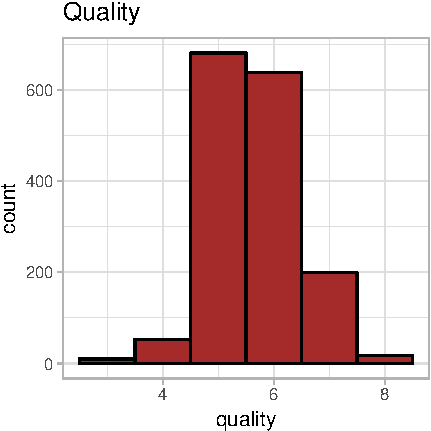
\includegraphics{P4-Analysis_of_a_dataset_files/figure-latex/Univariate_Plots-1.pdf}
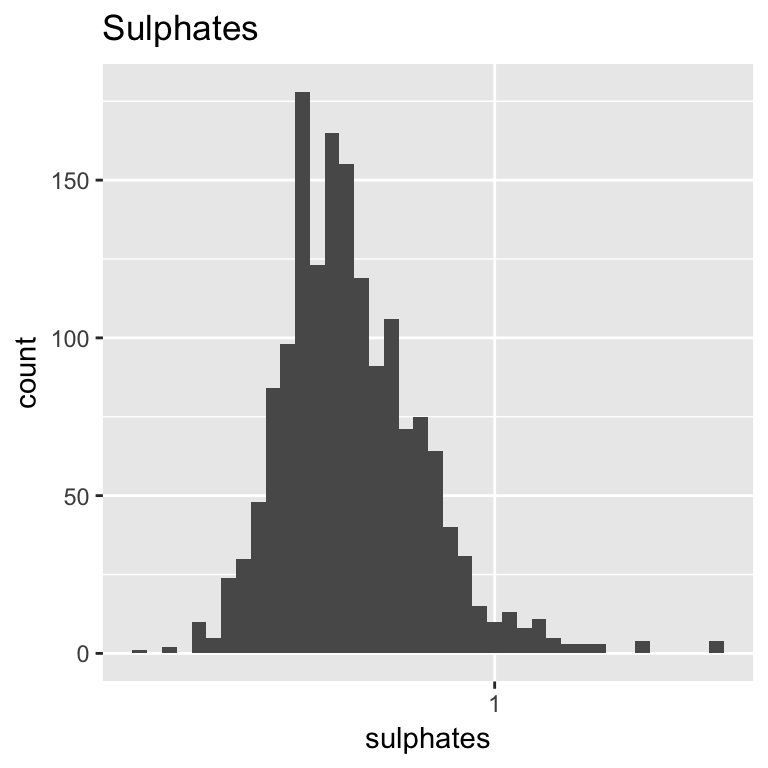
\includegraphics{P4-Analysis_of_a_dataset_files/figure-latex/Univariate_Plots-2.pdf}
\includegraphics{P4-Analysis_of_a_dataset_files/figure-latex/Univariate_Plots-3.pdf}

\subsection{Fixed and volatile
acidity}\label{fixed-and-volatile-acidity}

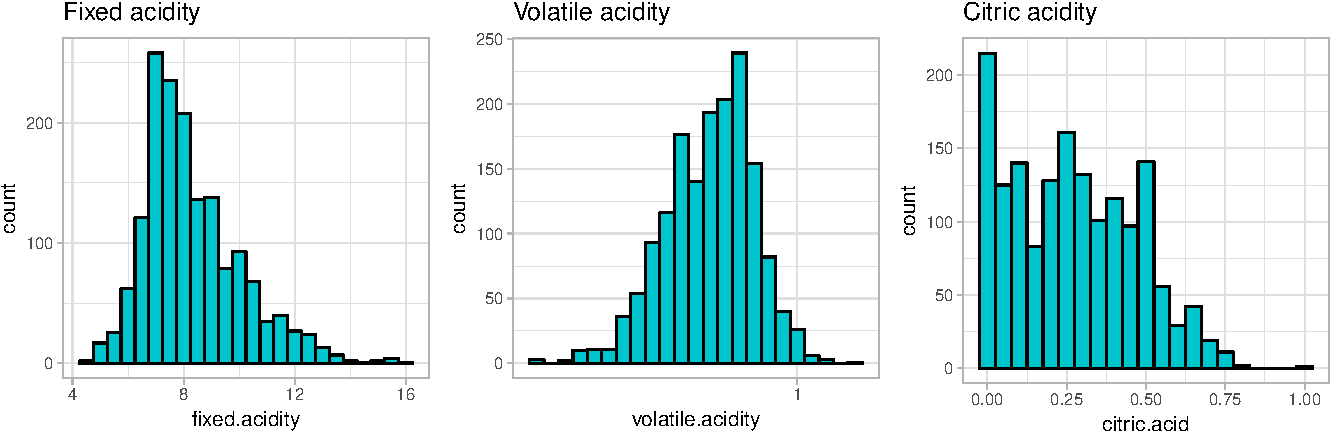
\includegraphics{P4-Analysis_of_a_dataset_files/figure-latex/Univariate_Plots_acidity-1.pdf}

\begin{verbatim}
## NULL
\end{verbatim}

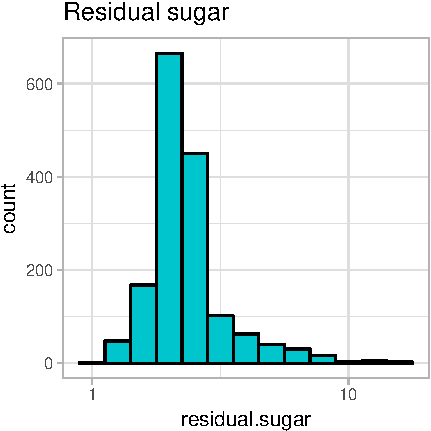
\includegraphics{P4-Analysis_of_a_dataset_files/figure-latex/Univariate_Plots_residual_sugar-1.pdf}

\begin{verbatim}
## NULL
\end{verbatim}

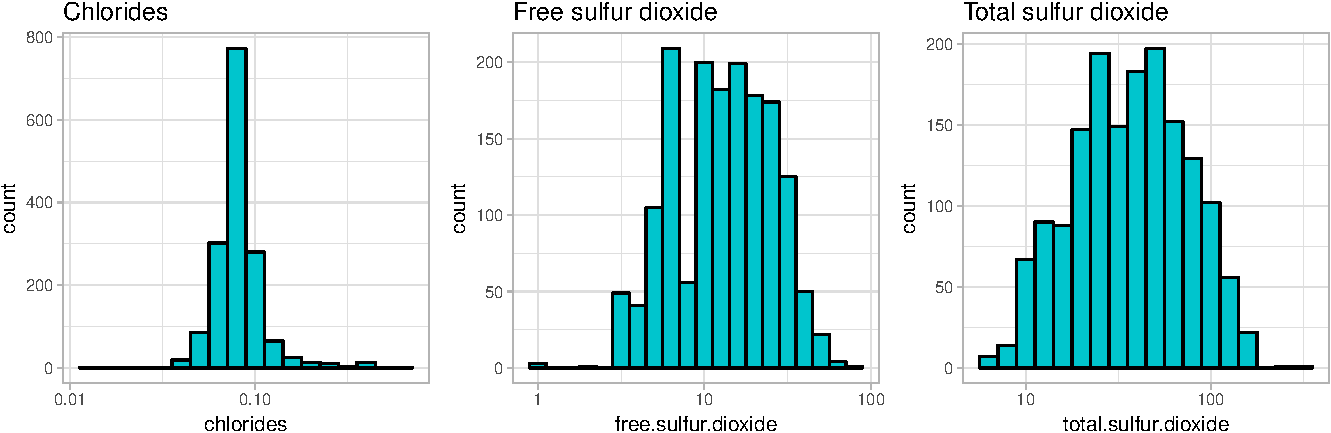
\includegraphics{P4-Analysis_of_a_dataset_files/figure-latex/Univariate_Plots_chlorides-1.pdf}

\begin{verbatim}
## NULL
\end{verbatim}

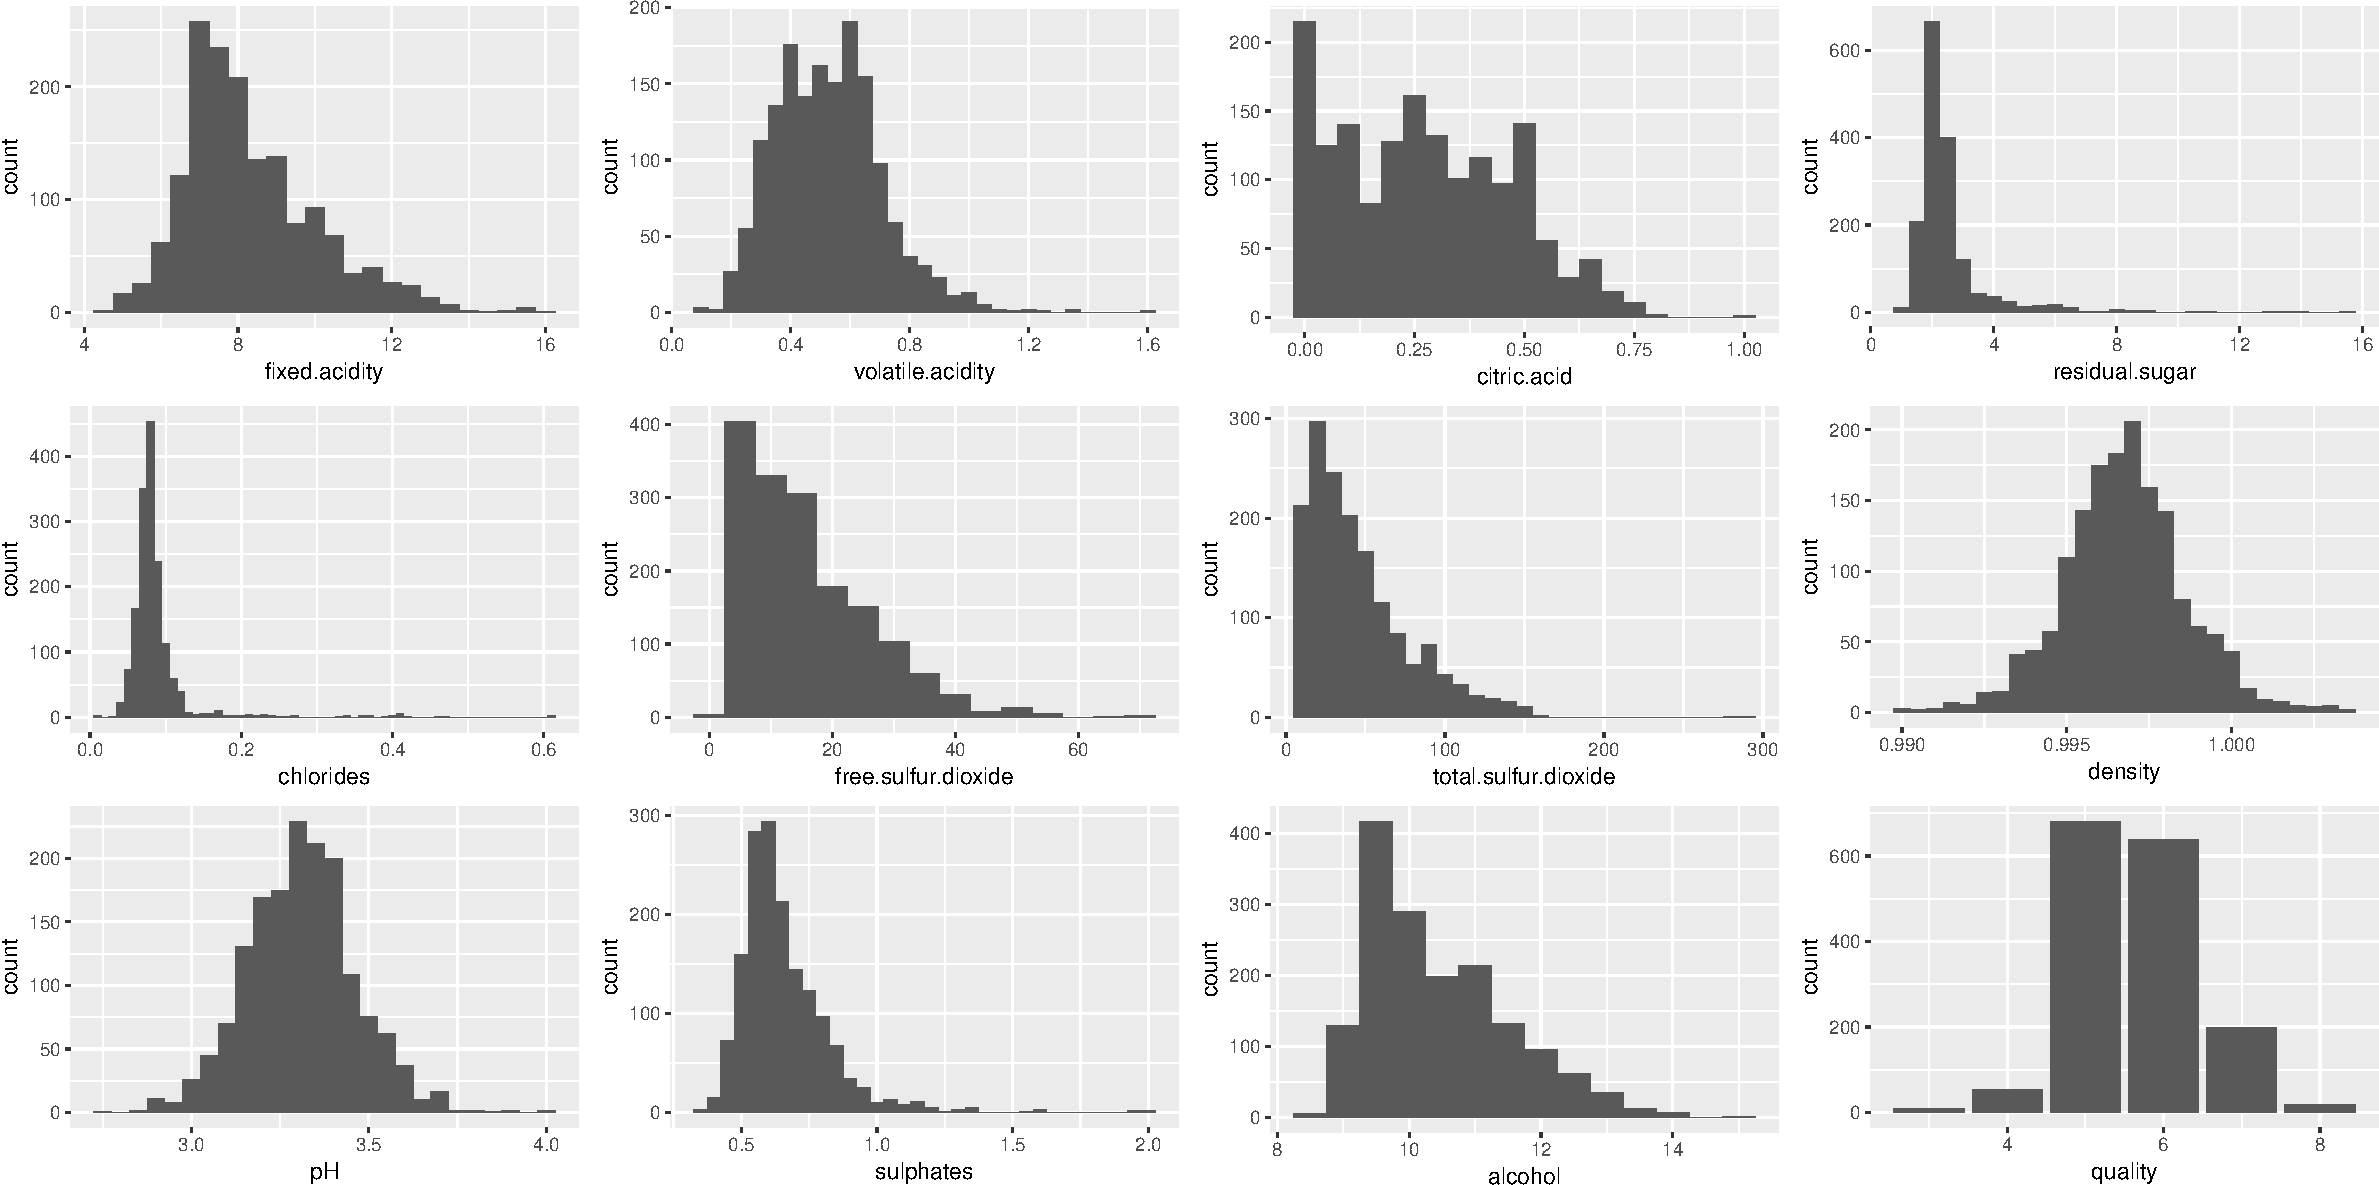
\includegraphics{P4-Analysis_of_a_dataset_files/figure-latex/Univariate_Plots_1-1.pdf}

\begin{verbatim}
## NULL
\end{verbatim}

\section{Univariate Analysis}\label{univariate-analysis}

\subsubsection{What is the structure of your
dataset?}\label{what-is-the-structure-of-your-dataset}

\subsubsection{What is/are the main feature(s) of interest in your
dataset?}\label{what-isare-the-main-features-of-interest-in-your-dataset}

\subsubsection{What other features in the dataset do you think will help
support your investigation into your feature(s) of
interest?}\label{what-other-features-in-the-dataset-do-you-think-will-help-support-your-investigation-into-your-features-of-interest}

\subsubsection{Did you create any new variables from existing variables
in the
dataset?}\label{did-you-create-any-new-variables-from-existing-variables-in-the-dataset}

\subsubsection{Of the features you investigated, were there any unusual
distributions? Did you perform any operations on the data to tidy,
adjust, or change the form of the data? If so, why did you do
this?}\label{of-the-features-you-investigated-were-there-any-unusual-distributions-did-you-perform-any-operations-on-the-data-to-tidy-adjust-or-change-the-form-of-the-data-if-so-why-did-you-do-this}

\section{Bivariate Plots Section}\label{bivariate-plots-section}

\section{Bivariate Analysis}\label{bivariate-analysis}

\subsubsection{Talk about some of the relationships you observed in this
part of the investigation. How did the feature(s) of interest vary with
other features in the
dataset?}\label{talk-about-some-of-the-relationships-you-observed-in-this-part-of-the-investigation.-how-did-the-features-of-interest-vary-with-other-features-in-the-dataset}

\subsubsection{Did you observe any interesting relationships between the
other features (not the main feature(s) of
interest)?}\label{did-you-observe-any-interesting-relationships-between-the-other-features-not-the-main-features-of-interest}

\subsubsection{What was the strongest relationship you
found?}\label{what-was-the-strongest-relationship-you-found}

\section{Multivariate Plots Section}\label{multivariate-plots-section}

\section{Multivariate Analysis}\label{multivariate-analysis}

\subsubsection{Talk about some of the relationships you observed in this
part of the investigation. Were there features that strengthened each
other in terms of looking at your feature(s) of
interest?}\label{talk-about-some-of-the-relationships-you-observed-in-this-part-of-the-investigation.-were-there-features-that-strengthened-each-other-in-terms-of-looking-at-your-features-of-interest}

\subsubsection{Were there any interesting or surprising interactions
between
features?}\label{were-there-any-interesting-or-surprising-interactions-between-features}

\subsubsection{OPTIONAL: Did you create any models with your dataset?
Discuss the strengths and limitations of your
model.}\label{optional-did-you-create-any-models-with-your-dataset-discuss-the-strengths-and-limitations-of-your-model.}

\begin{center}\rule{0.5\linewidth}{\linethickness}\end{center}

\section{Final Plots and Summary}\label{final-plots-and-summary}

\subsubsection{Plot One}\label{plot-one}

\subsubsection{Description One}\label{description-one}

\subsubsection{Plot Two}\label{plot-two}

\subsubsection{Description Two}\label{description-two}

\subsubsection{Plot Three}\label{plot-three}

\subsubsection{Description Three}\label{description-three}

\begin{center}\rule{0.5\linewidth}{\linethickness}\end{center}

\section{Reflection}\label{reflection}

\section{Others}\label{others}

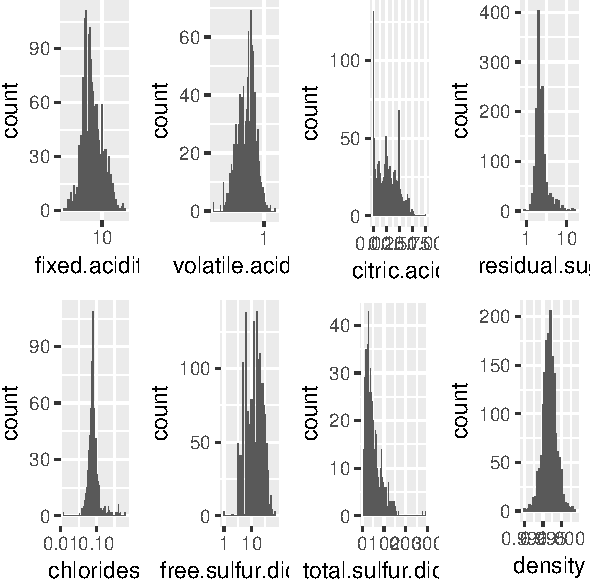
\includegraphics{P4-Analysis_of_a_dataset_files/figure-latex/Univariate_Plots_log-1.pdf}

\begin{verbatim}
## NULL
\end{verbatim}

\bibliography{P4.bib}


\end{document}
